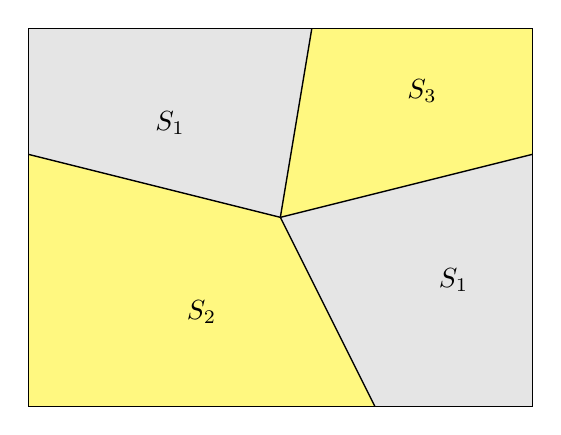
\begin{tikzpicture}[scale=0.8]
  %–– Regioni ––
  % S1 sinistro
  \fill[gray!20]
    (4,3) -- (0,4) -- (0,6) -- (4.5,6) -- cycle;
  % S3 (giallo)
  \fill[yellow!50]
    (4,3) -- (4.5,6) -- (8,6) -- (8,4) -- cycle;
  % S1 destro
  \fill[gray!20]
    (4,3) -- (8,4) -- (8,0) -- (5.5,0) -- cycle;
  % S2 (azzurro)
  \fill[yellow!50]
    (4,3) -- (5.5,0) -- (0,0) -- (0,4) -- cycle;

  %–– Confini interni spessi blu ––
  \draw[black, line width=0.5pt] (4,3) -- (0,4);
  \draw[black, line width=0.5pt] (4,3) -- (4.5,6);
  \draw[black, line width=0.5pt] (4,3) -- (8,4);
  \draw[black, line width=0.5pt] (4,3) -- (5.5,0);

  %–– Bordo esterno ––
  \draw[black, line width=0.5pt] (0,0) rectangle (8,6);

  %–– Etichette ––
  \node at (2.25,4.5) {$S_1$};
  \node at (2.75,1.5) {$S_2$};
  \node at (6.25,5) {$S_3$};
  \node at (6.75,2) {$S_1$};
\end{tikzpicture}
